\usepackage{etex} %эта магическая херь избавляет от переполнения регистров TeX а!!!

\mode<article>{\usepackage{fullpage}}
\mode<presentation>{
    \usetheme{Madrid}
    \useoutertheme{shadow}
} 

\usepackage[utf8]{inputenc}
\usepackage[russian]{babel}
\usepackage{indentfirst}
\usepackage{graphicx}

\usepackage{amsmath}
\usepackage{amsfonts}
\usepackage{amsthm}
%\usepackage{algorithm}
%\usepackage{algorithmic}

%\usepackage[all]{xy}

\date{Лекция по дисциплине <<методы и средства защиты компьютерной информации>> (\today)}
\author[М.~М.~Шихов]{Михаил Шихов \\ \texttt{\underline{m.m.shihov@gmail.com}}}

%%для рисования графов пакетом xy-pic
%\entrymodifiers={++[o][F-]}

%%для псевдокода алгоритмов (algorithm,algorithmic)
%\renewcommand{\algorithmicrequire}{\textbf{Вход:}}
%\renewcommand{\algorithmicensure}{\textbf{Выход:}}
%\renewcommand{\algorithmiccomment}[1]{// #1}
%\floatname{algorithm}{Псевдокод}

%\setbeamercolor{alerted text}{fg=-green} %gyan, blue, green, -green

\title[Биометрическая аутентификация]{Методы аутентификации.\\Биометрические методы.\\Признаки <<чем является>>, <<что умеет>>}


\begin{document}


%титул и содержание статьи
\mode<article>{\maketitle\tableofcontents}

%титул и содержание презентации
\frame<presentation>{\titlepage}
\begin{frame}<presentation>
    \frametitle{Содержание}
    \tableofcontents
\end{frame}


\section{Аутентификация}


\subsection{Основы}


\begin{frame}
\frametitle{Аутентификация}
\begin{definition}%theorem, lemma, proof, corollary, example
\alert{Аутентификация} --- это проверка подлинности
\end{definition}
Аутентификация может быть произведена на основе проверки следующих признаков.
\begin{enumerate}
    \item Something you know (Что знает).
    \item Something you have (Что имеет).
    \item \alert{Something you are (Чем является)}.
    \item \alert{Something you can (Что умеет)}.
\end{enumerate}
Далее сосредоточим внимание на последних двух признаках, на которых основана биометрическая аутентификация.
\end{frame}


\begin{frame}
\frametitle{Аутентичность}
Возникает необходимость в аутентификации всех компонент информационной системы:
\begin{itemize}
    \item \alert{персонала};
    \item \alert{клиентов} (их автоматизированных систем);
    \item \alert{поставшиков} (их автоматизированных систем);
    \item программных и программно-аппаратных средств;
    \item данных.
\end{itemize}
В данном случае мы сосредоточимся на аутентификации \alert{пользователя}, как уникального биологического существа.
\end{frame}


\section{Биометрическая аутентификация}


\subsection{Определение}


\begin{frame}
\frametitle{Биометрическая аутентификация}
\begin{definition}%theorem, lemma, proof, corollary, example
    \alert{Биометрическая} аутентификация человека основана на измерении его уникальных биологических параметров и сопоставлении их с образцом.
\end{definition}
Различают две рабочие фазы (режима).
\begin{enumerate}
    \item Регистрации. 
    \mode<article>{Проведение измерений биологических параметров, с целью получения эталонного образца для базы учетных записей. Обычно объем биометрических данных велик, и эталон (эталоны) представляют собой результат их предварительной обработки (например, шумоочистки, устранения избыточности и т.д.)}
    
    \item Аутентификация.
    \mode<article>{Проведение измерений биологических параметров, с целью сопоставления с полученым на этапе регистраци  эталонным образцом и принятия решения о результатах аутентификации.}
\end{enumerate}
Система биометрической аутентификации состоит из подсистем.
\begin{itemize}
    \item Измерения (сканер).
    \mode<article>{Получение данных замера и их предобработка.}
    
    \item Идентификации.
    \mode<article>{Назначает пользователю идентификатор, который получен в процессе сопоставления эталонов с замером (аутентификации). Либо пользователь предъявляет идентификатор сам, и аутентификация (сверка с эталоном) выполняется уже адресно, а не по всей базе учетных записей.}
    
    \item Аутентификации.
    \mode<article>{Сверка замера с эталоном.}
    
    \item Регистрации.
    \mode<article>{Прведение измерений с целью формирования эталонов для базы учетных записей.}
\end{itemize}
\end{frame}


\subsection{Параметры}

\begin{frame}
\frametitle{Параметры систем биометрической аутентификации}
\begin{itemize}

    \item FRR (False Rejection Rate). Коэффициент (вероятность) ошибочного отказа. $\leq 10^{-2}$.
    \mode<article>{Отказано в доступе законному пользователю.}
    
    \item FAR (False Acceptance Rate). Коэффициент (вероятность) ошибочного подтверждения подлинности. $\leq 10^{-4}$.
    \mode<article>{Подтверждение личности незаконного пользователя.}
    
\end{itemize}
\end{frame}


\subsection{Классы}

\begin{frame}
\frametitle{Классы методов биометрической аутентификации}
\begin{itemize}
    \item Статические (физиологические).
    
    Черты лица, рисунок радужной оболочки глаза, рисунок кровеносных сосудов сетчатки глаза, параметры пальцев (папиллярные линии, рельеф, длина суставов и т.д.), форма ладони, рисунок вен на запястье, тепловая картина и т.д. 
    \mode<article>{
    Проверка ведется по неотъемлемой, уникальной характеристике, данной человеку от рождения. Здесь анализируются такие признаки, как черты лица, структура глаза (сетчатки или радужной оболочки), параметры пальцев (папиллярные линии, рельеф, длина суставов и т. д.), ладонь (ее отпечаток или топография), форма руки, рисунок вен на запястье или тепловая картина. 
    }
    
    \item Динамические (поведенческие, психологические).
    
    Голос человека, особенности рукописной подписи, динамические параметры в процессе письма, особенности ввода текста с клавиатуры, работы с манипулятором типа <<мышь>>.
    \mode<article>{
    Методы используют особенности, характерные для подсознательных движений в процессе воспроизведения человеком какого-либо действия. К таким особенностям относятся голос человека, особенности его подписи, динамические параметры письма, особенности ввода текста с клавиатуры и т.д.
    }
    
\end{itemize}
\end{frame}


\begin{frame}[allowframebreaks]
\frametitle{Дактилоскопические системы. Fingerprint identification}
\framesubtitle{Статические методы}

\begin{figure}
    \begin{center}
        \mode<presentation>{ 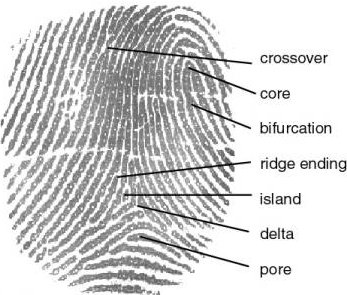
\includegraphics[height=.4\textheight]{pict/fingerprint} }
        \mode<article>{ 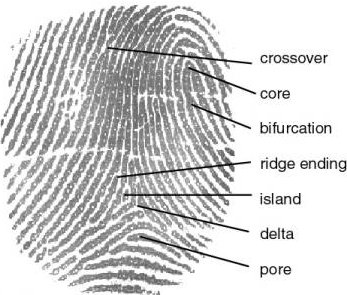
\includegraphics[width=.4\textwidth]{pict/fingerprint} } 
    \end{center}
\end{figure} 

\begin{itemize}
    \item Автоматизация началась с 1960-х гг.
    \item Используются полицией (государственные и банковские системы). Большие базы данных (FBI).
    \item Типы сканеров: оптические, емкостные, ультразвуковые, термические.
    \item Два типа методов сопоставления: pattern matching, minutiae-based matching.
    \item minutiae --- микроточка, особенность папиллярной линии (пересечение (crossover), центр, ядро, разветвление, окончание, островок, дельта, впадина). Фиксируется тип minutiae и его расположение.
    \item AFIS\footnote{Automated Fingerprint Identification System} активно используют minutiae-based matching.
    \item Устойчивость к обману --- измеряются физические параметры кожи пальца.
    \item Стандартизация: форматы обмена данными (ANSI/INCITS: 381-2004, 377-2004, 378-2004; ISO/IEC 19794-2, 19794-3, 19794-4\footnote{Имеются соответствующие ГОСТ Р ИСО/МЭК 19794-X}) 
    \item FAR=0.
    \item Низкий уровень дискомфорта.
    \item Оптические методы чувствительны к загрязнению поверхности пальцев.
    \item Папиллярный узор имеет свойство восстанавливаться после повреждения кожных покровов. 
    \item Псориаз --- болезнь, повреждающая кожные покровы.
    \item Психологическое предубеждение: ассоциации с криминальной сферой.
    \item Сложно использовать без ведома пользователя.
\end{itemize}
\end{frame}


\begin{frame}[allowframebreaks]
\frametitle{Форма ладони. Hand Geometry Recognition}
\framesubtitle{Статические методы}

\begin{figure}
    \begin{center}
        \mode<presentation>{ 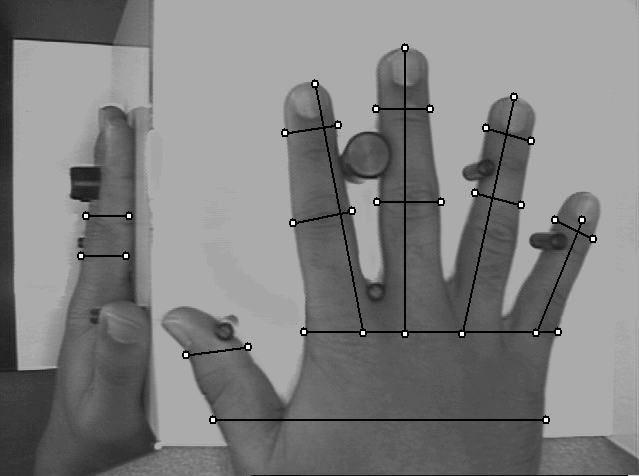
\includegraphics[height=.4\textheight]{pict/handrec} }
        \mode<article>{ 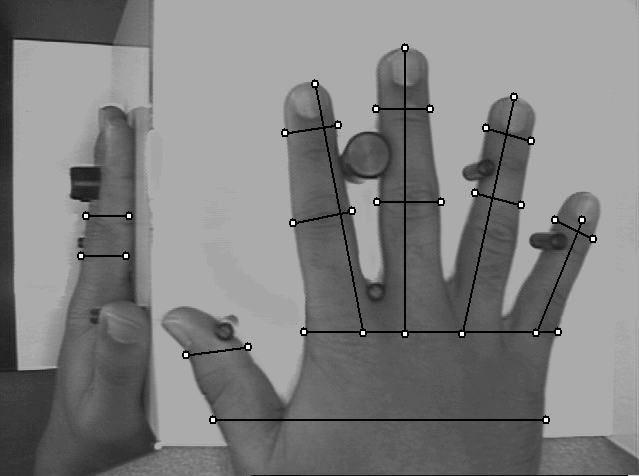
\includegraphics[width=.4\textwidth]{pict/handrec} } 
    \end{center}
\end{figure} 

\begin{itemize}
    \item Выход на рынок в 1980-х гг.
    \item Активно применяются для систем контроля посещаемости, физического доступа.
    \item Тип сканера --- CCD (ПЗС) камера.
    \item Производятся замеры: длины и толщины пальцев, толщину и площадь поверхности ладони.
    \item Устойчивость к обману --- измеряются физические параметры кожи ладони.
    \item Стандартизация: форматы обмена данными (ISO/IEC 19794-10) 
    \item Относительно большие габариты сканера.
    \item Низкий уровень FAR.
    \item Низкий уровень дискомфорта.
    \item Психологическое предубеждение отсутствует.
    \item Сложно использовать без ведома пользователя.
\end{itemize}
\end{frame}


\begin{frame}[allowframebreaks]
\frametitle{Изображение сосудистого русла. Vascular Pattern Recognition}
\framesubtitle{Статические методы}

\begin{figure}
    \begin{center}
        \mode<presentation>{ 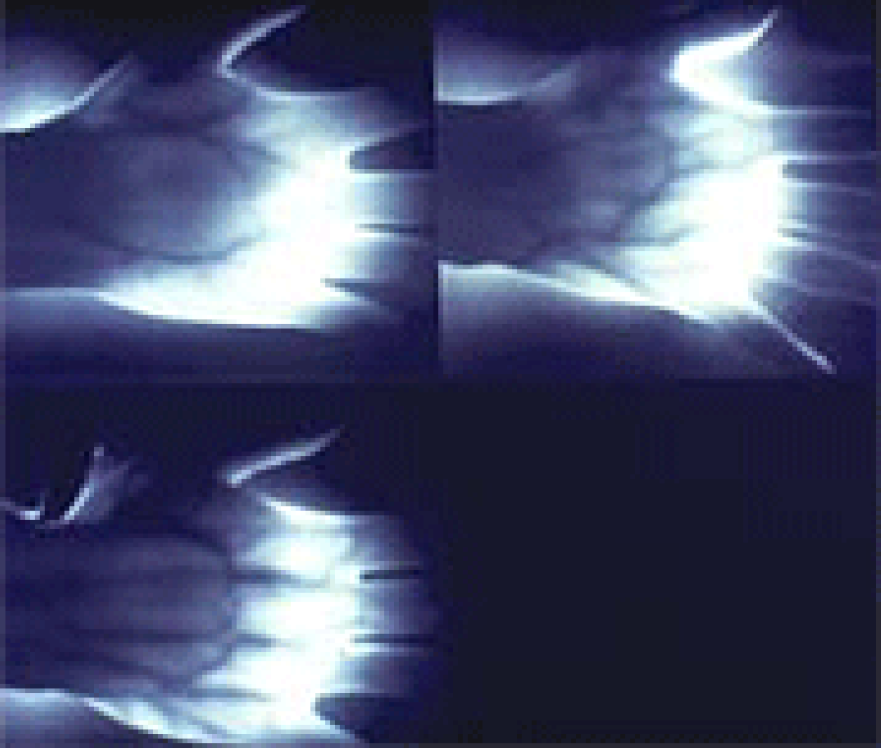
\includegraphics[height=.4\textheight]{pict/veins} }
        \mode<article>{ 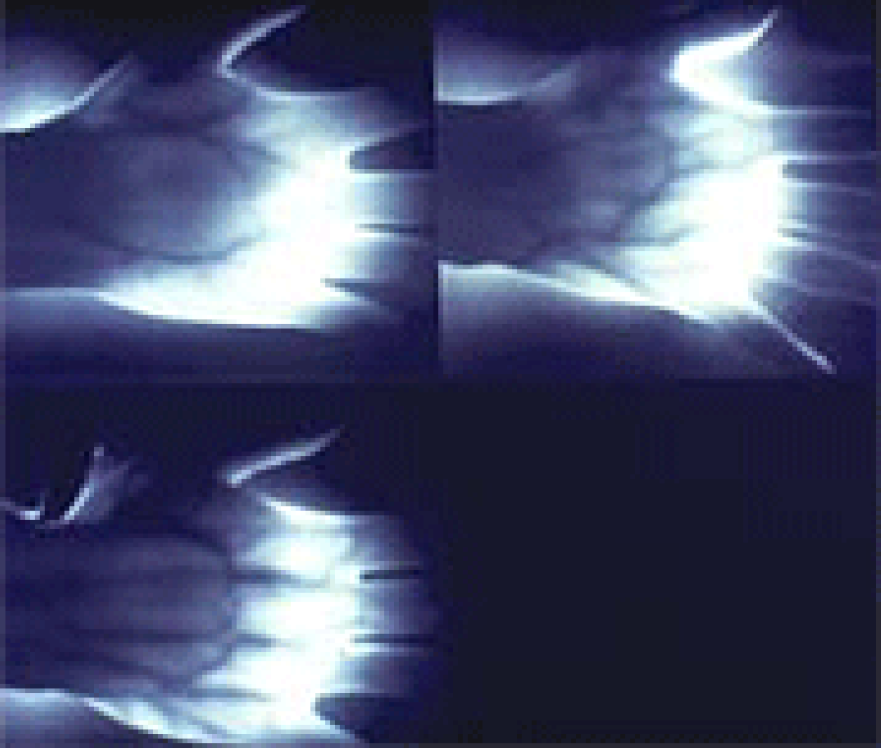
\includegraphics[width=.4\textwidth]{pict/veins} } 
    \end{center}
\end{figure} 

\begin{itemize}
    \item Возможность обсуждалась с 1992 г. Исследовательские статьи опубликованы в 2000 гг. 
    \item 1:1, 1:m идентификация.
    \item Используются в банкоматах, больницах и университетах (преимущественно в японии).
    \item Изображение вен получается при освещении близким к инфракрасному излучением.
    \item Фиксируются толщина вен, точки ветвления, углы ветвления и т.д.
    \item Устойчивость к обману кровь должна течь по венам.
    \item Стандартизация: форматы обмена данными (ISO/IEC 19794-9\footnote{Имеются соответствующие ГОСТ Р ИСО/МЭК 19794-X}) 
    \item Близкий к нулю FAR.
    \item Низкий уровень дискомфорта. Не требуется контакт с поверхностью.
    \item Рисунок вен практически не меняется с возрастом.
    \item Сложно использовать без ведома пользователя.
\end{itemize}
\end{frame}


\begin{frame}[allowframebreaks]
\frametitle{Радужная оболочка глаза. Iris Recognition}
\framesubtitle{Статические методы}

\begin{figure}
    \begin{center}
        \mode<presentation>{ 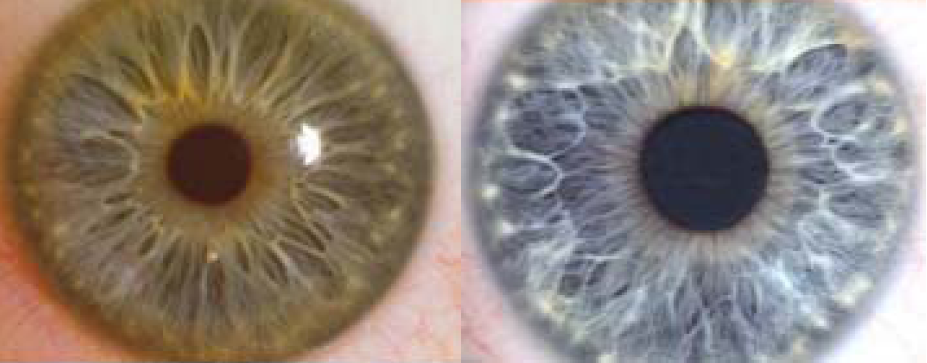
\includegraphics[height=.4\textheight]{pict/iris} }
        \mode<article>{ 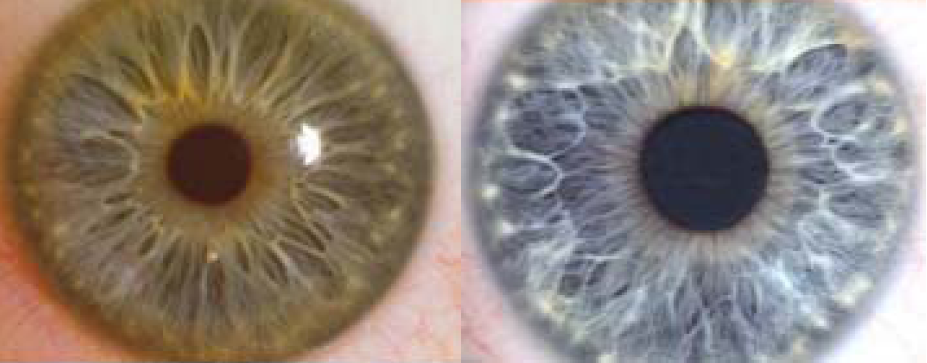
\includegraphics[width=.4\textwidth]{pict/iris} } 
    \end{center}
    \caption{Радужная оболочка}\label{pict:iris}
\end{figure} 

\begin{figure}
    \begin{center}
        \mode<presentation>{ 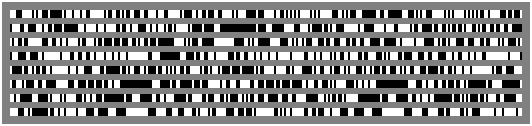
\includegraphics[height=.25\textheight]{pict/iriscode} }
        \mode<article>{ 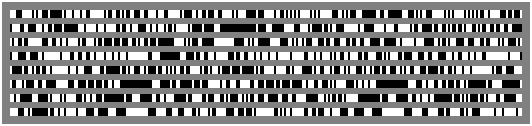
\includegraphics[width=.4\textwidth]{pict/iriscode} } 
    \end{center}
    \caption{IrisCode\textregistered}\label{pict:iriscode}
\end{figure} 

\begin{itemize}
    \item Возможность обсуждалась с 1936 г. В 1995 г. первые аппаратные реализации.
    \item Используются в основном военными и на объектах оборонного значения.
    \item Изображение получается инфракрасной камерой.
    \item В IrisCode\textregistered\footnote{Изобретатель --- Джон Даугман, патент заканчивается в 2011 г.} --- простое расстояние Хемминга двух IrisCode\textregistered.
    \item Устойчивость к обману.
    \item Стандартизация: форматы обмена данными (ISO/IEC 19794-6\footnote{Имеются соответствующие ГОСТ Р ИСО/МЭК 19794-X}) 
    \item FAR$\leq 10^{-78}$.
    \item Низкий уровень дискомфорта.
    \item Дорогостоящее оборудование.
    \item Психологическое предубеждение отсутствует.
    \item Сложно использовать без ведома пользователя.
\end{itemize}
\end{frame}




\begin{frame}[allowframebreaks]
\frametitle{Черты лица. Face Recognition}
\framesubtitle{Статические методы}

\begin{itemize}
    \item Разработка началась с 1960-х гг.
    \item Методы активно разрабатываются, так как не требует согласия пользователя.
    \item В качестве сканера используется фото-видео аппаратура.
    \item Три главных класса алгоритмов: Метод главных компонент (Principal component analysis (PCA)), Дискриминантный анализ (Linear discriminant analysis (LDA)), Сравнение графов с эластичными связями (Elastic Bunch Graph Matching (EBGM)).
    \item Стандартизация: форматы обмена данными (ISO/IEC 19794-5\footnote{Имеются соответствующие ГОСТ Р ИСО/МЭК 19794-X}) 
    \item Низкий FAR.
    \item Относительно дешевая аппаратура (используются стандартные устройства).
    \item Дискомфорт отсутствует.
    \item Психологическое предубеждение перед возможностями тотального контроля.
    \item Можно использовать без ведома пользователя.
\end{itemize}
\end{frame}


\begin{frame}[allowframebreaks]
\frametitle{Динамические методы}
\framesubtitle{Голос. Speaker, Voice Recognition}

\begin{figure}
    \begin{center}
        \mode<presentation>{ 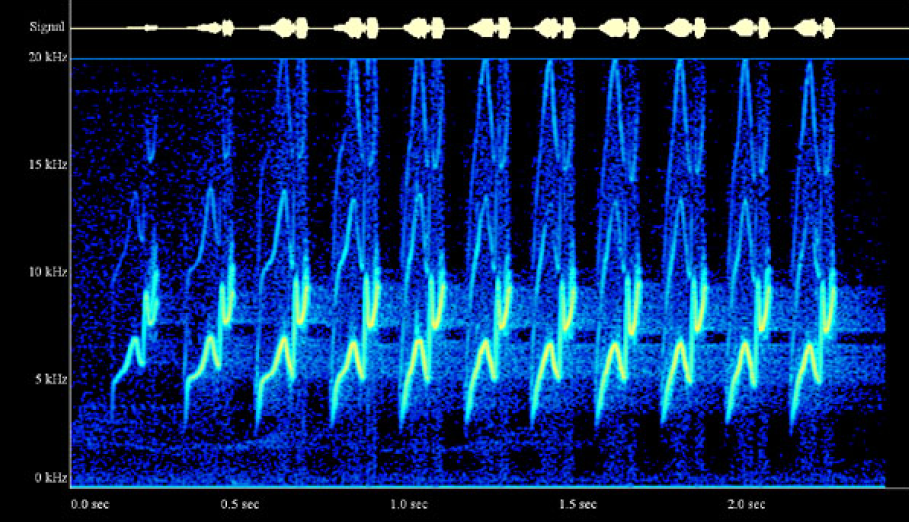
\includegraphics[height=.4\textheight]{pict/voice} }
        \mode<article>{ 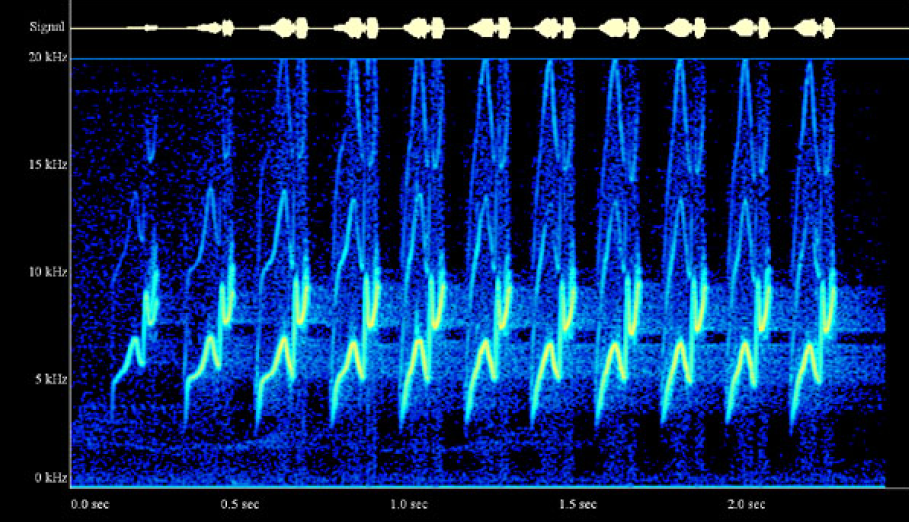
\includegraphics[width=.4\textwidth]{pict/voice} } 
    \end{center}
\end{figure} 

\begin{itemize}
    \item Разработка ведется с 1960-х гг.
    \item Редко используется в однофакторном варианте. Часто применяется для аутентификации в приложениях телефонии.
    \item В качестве сканера используется практически любой микрофон.
    \item Не путать с распознаванием речи!
    \item Два типа: Зависимые от образца (text dependent) и независимые (text independent).
    \item Алгоритмы используют уникальные особенности голоса: тембр, высоту, модуляцию, частоту, громкость.
    \item Голос легко записать. Поэтому методы используются только в виде challenge-response (т.е. пользователя просят повторить случайную фразу или воспроизнести надпись экране\ldots).
    \item Стандартизация: INCITS 398-2005 в общем виде определяет элементы для описания биометрических данных, но не содержит частностей, касающихся распознования голоса.
    \item Низкий FAR.
    \item Одна из самых дешевых систем с точки зрения затрат на аппаратуру.
    \item FRR сильно зависит от состояния здоровья пользователя. Например, простудные заболевания влияют на голос.
    \item Психологическое предубеждение отсутствует.
    \item Можно использовать без ведома пользователя.
\end{itemize}
\end{frame}


\begin{frame}[allowframebreaks]
\frametitle{Подпись. Dynamic Signature}
\framesubtitle{Динамические методы}

\begin{itemize}
    \item Разработка (статические хар-ки подписи: форма) началась с 1965 г. С 1977 г. разработка <<динамических>> (ускорения, характер письма, нажим) методов.
    \item Используются преимущественно в банковских системах.
    \item Обычно в трех измерениях X,Y,Z производятся замеры скорости, ускорения, ритма, давления, направления с помощью планшета или ручки с пьезоэлектрическими датчиками.
    \item Высокая устойчивость к обману.
    \item Стандартизация: форматы обмена данными (ANSI/INCITS: 395-2005; ISO/IEC 19794-7,19794-11\footnote{Имеются соответствующие ГОСТ Р ИСО/МЭК 19794-X}) 
    \item Низкий FAR. Достаточно большой процент FRR.
    \item Низкий уровень дискомфорта.
    \item Психологическое предубеждение отсутствует.
    \item Сложно использовать без ведома пользователя.
\end{itemize}
\end{frame}



\section{Комбинированные технологии}


\subsection{Биоэлектронные системы}


\begin{frame}
\frametitle{Биоэлектронные системы}
Двухфакторная аутентификация на сочетающая в себе биометрическую систему и признак <<что имеет>>.
\begin{enumerate}
    \item Пользователь вставляет в считыватель аутентичный носитель зашифрованных биометрических данных (чип-карту, usb-ключ,\ldots).
    \item Проводится биометрическая процедура, результаты которой сверяются с расшифрованными данными с носителя (обычно дактилоскопическая).
\end{enumerate}
Достоинства:
\begin{enumerate}
    \item Простота и удобство использования для конечного пользователя.
    \item Высокий уровень защищенности.
    \item Аппаратная реализация криптографических преобразований.
\end{enumerate}
\end{frame}


\section{Стандарты в области биометрии}


\subsection{Биометрические стандарты}


\begin{frame}[allowframebreaks]
\frametitle{Биометрические стандарты определяют}
\begin{enumerate}
    \item Интерфейсы технических систем (ISO/IEC 24708 --- BioAPI Interworking Protocol).
    \item Форматы для обмена биометрическими данными (CBEFF --- Common Biometric Exchange File Format, ISO/IEC 19794-X --- Biometric data interchange formats).
    \item Прикладные программные интерфейсы (ISO/IEC 19784-1 --- Biometric Application Programming Interface).
    \item Метрики производительности (ISO/IEC 19795-X --- Biometric performance testing and reporting).
    \item Подходы к тестированию производительности и требования к результатам тестов (ISO/IEC 19795-X --- Biometric performance testing and reporting).
\end{enumerate}
\end{frame}


\appendix %приложения


\begin{frame}
    \frametitle{Источники}
    Общее описание методов биометрической аутентификации можно найти в \cite{bib:chmora:crypto,bib:shangin:protect}.

    Подробно о биометрии: \cite{bib:misc:biocons,bib:misc:ibg,bib:misc:bioapi}.

    Стандарты: \cite{bib:misc:iso,bib:misc:incits}.

    Рекомендованы к прочтению: ГОСТ Р ИСО/МЭК 19794 (эквиваленты соотв. стандартов ISO/IEC). Страничка разработчика метода аутентификации по радужной оболочке глаза: \cite{bib:misc:daugmann}. Аутентификация на основе черт лица: \cite{bib:misc:facerec}.
\end{frame}


\begin{frame}[allowframebreaks]{Библиография}
    \bibliographystyle{gost780u}
    \bibliography{./../bibliobase}
\end{frame}


\end{document}